\newpage

\section{Literature Review}
Various studies have explored different approaches to designing robots that can autonomously navigate
hospital environments and assist in routine medical tasks like delivering medicine. This literature review
examines the current state of research and development projects relevant to this aspect of robot navigation
and in the light of the healthcare industry. 



\subsection{Overview of Navigation in Robotics}
\noindent Navigation encompasses the ability of a robot to act based on its knowledge and sensor data so as to reach its goal
position as efficiently and reliably as possible. In~\cite{ozkil2009navigation}, robotics has conventionally been
hierarchical, in that it consists of a dynamical control loop with integration of four key components: Perception, Localization, Cognition, and Motion
Control as depicted in \figref{nav_overview} below. Perception involves gathering data from the environment using sensors like cameras, LIDAR, and ultrasonic sensors,
enabling the robot to understand its surroundings and detect obstacles. Localization is the process of determining the 
robot`s position within its environment. Cognition refers to the decision-making process, where the robot interprets data from perception
and localization to plan its path, avoid obstacles, and adapt to changes in real-time. Motion Control involves
executing the navigation plan by converting cognitive decisions into motor commands. Together, these components create
a cohesive system that allows robots to navigate autonomously and effectively in complex environments.

\vspace{1.0em}

\begin{figure}[H]
    \centering
    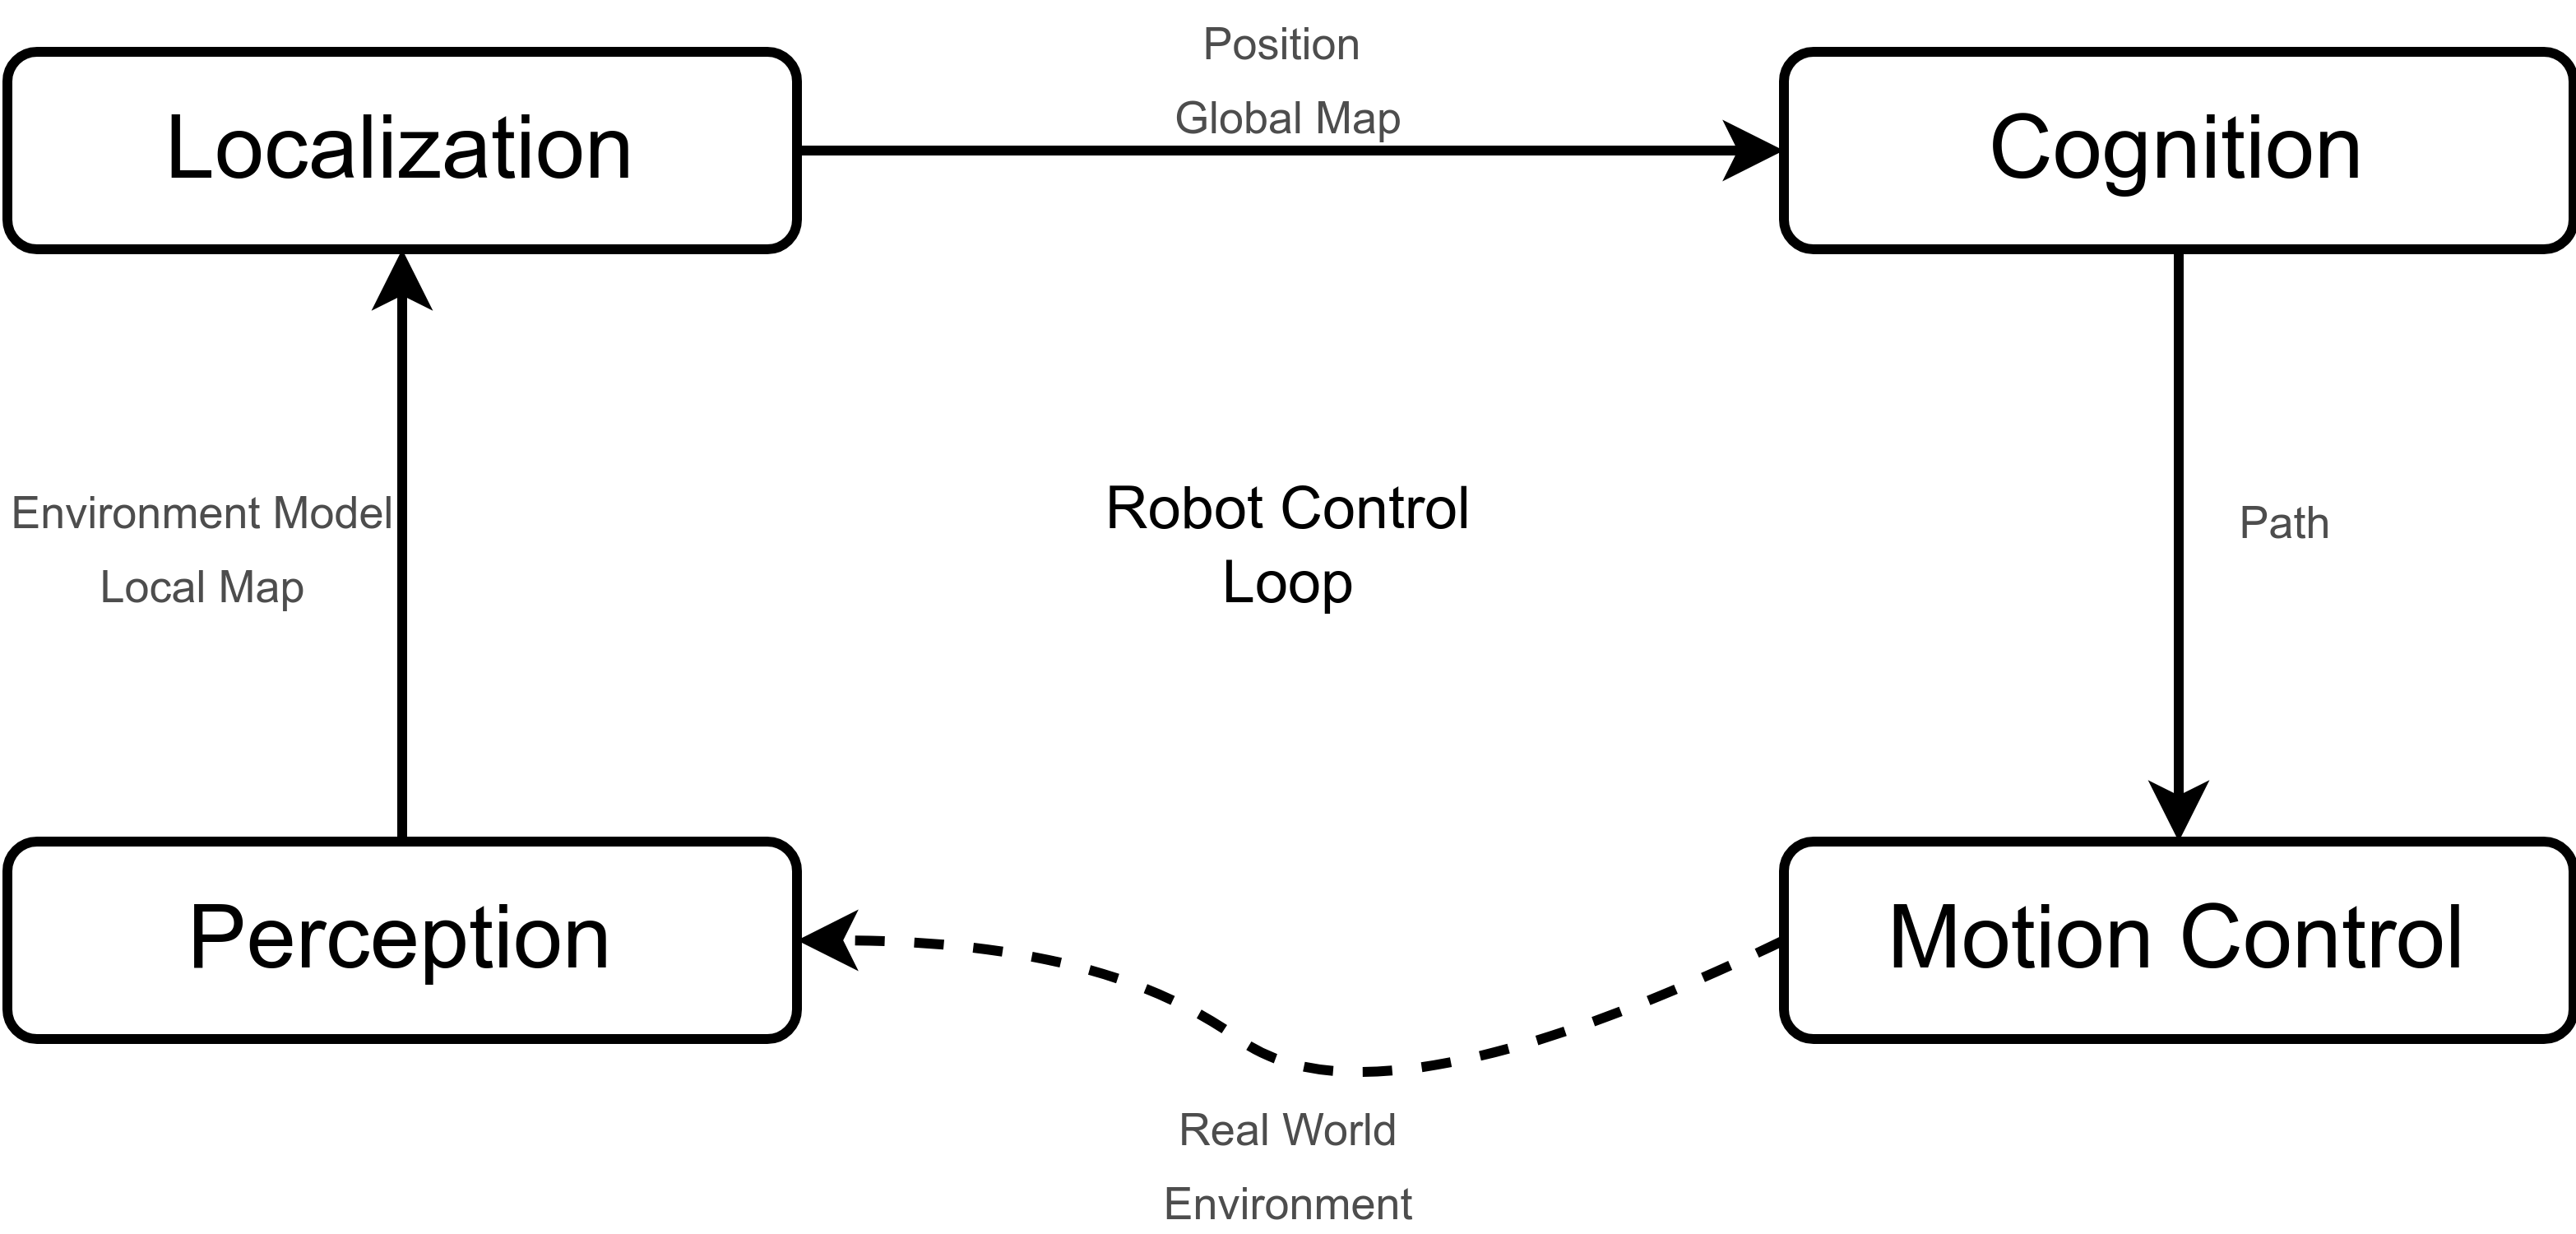
\includegraphics[width=4.6in, height=2.8in]{pics/navigation_overview.png}
    \caption[Overview of Navigation Problem]{Overview of Navigation Problem~\cite{ozkil2009navigation}}\label{nav_overview}
\end{figure}



\subsection{Localization and Mapping}
Localization is the process of determining the robot's position in the environment while mapping involves creating an internal
model of any unknown features in the environment~\cite{riisgaard2006slam}. Since both these processes are interdependent, a question arises whether it is
possible for a robot to perform self-localization when placed in an unknowned environment. This is widely referred to as
Simultaneous Localization and Mapping (SLAM) as Durrant Whyte depicts it in~\cite{durrant-whyte2006slam1} a ``holy grail'' for making the
dream of autonomous mobile robot come true. Researchers recently have proposed various algorithms to achieve SLAM in robot navigation and
as since some of these algorithms share similar steps in their design, there are many approaches to categorizing the techniques used in SLAM.\@
SLAM can be broadly categorized into two types based on the scale of localization:
\begin{enumerate}
    \item \textit{Global SLAM:} ability to determine the robot's position in an previously learned map, given no other information than
    that the robot is somewhere in the map.
    \item \textit{Local SLAM:} ability to track the robot's position over time, given that the robot's initial position is known (localized).
\end{enumerate}

\subsubsection{Dead Reckoning}
Dead reckoning is simple method that estimates the robot's current position based on its previously known position. The
position is determined using data from wheel encoders and inertial sensors like gyroscopes and accelerometers~\cite{borenstein1997mobile}.
While easy to implement and computationally efficient, dead reckoning can draw so many errors due to wheel slippage, uneven terrain, and
sensor noises or inaccuracies.This makes it unreliable for long-term navigation in unknown environments~\cite{PARK1998219}.
\subsubsection{Kalman Filters}
Kalman filters are recursive algorithms used to estimate the state of a dynamic system from a series of incomplete and noisy
measurements~\cite{thrun2005probabilistic}.\@ The foundation of KF is Bayes`s theorem, which combines prior knowledge of robot's position with new measurements to update
the estimate.
KF assumes that the system model is linear and the noise is Gaussian, which is represented by a normal distribution.
real-world scenarios. \\

\vspace{-0.2em}
\begin{itemize}
    \item \textbf{Prediction Step:}
    \begin{equation}
        \mu_{t|t-1} = A \mu_{t-1} + B u_{t-1}
    \end{equation}
    \vspace{-2.5em}
    \begin{equation}
        \Sigma_{t|t-1} = A \Sigma_{t-1} A^T + Q_t
    \end{equation}
    \vspace{-2.5em}
    
    where:
    \vspace{-0.3em}
    \begin{itemize}
        \item $\mu_{t|t-1}$ is the predicted state at time $t$.
        \item $\Sigma_{t|t-1}$ is the predicted covariance matrix.
        \item $A$ is the state transition model.
        \item $B$ is the control input model.
        \item $Q_t$ is the process noise covariance.
    \end{itemize}

    \item \textbf{Update Step:}
    \begin{equation}
        K_t = \Sigma_{t|t-1} C^T {\left(C \Sigma_{t|t-1} C^T + R_t\right)}^{-1}
    \end{equation}
    \vspace{-2.5em}
    \begin{equation}
        \mu_t = \mu_{t|t-1} + K_t (z_t - C \mu_{t|t-1})
    \end{equation}
    \vspace{-2.5em}
    \begin{equation}
        \Sigma_t = (I - K_t C) \Sigma_{t|t-1}
    \end{equation}
    \vspace{-1.5em}
    where:
    \vspace{0.5em}
    \begin{itemize}
        \item $K_t$ is the Kalman gain.
        \item $C$ is the observation model.
        \item $R_t$ is the measurement noise covariance.
        \item $z_t$ is the actual measurement update.
        \item $\delta_t \sim N(0, R_t)$ represents measurement noise.
    \end{itemize}
\end{itemize}

\begin{comment}
\textbf{Observation Model for KF:}
\begin{equation}
    z_t = C \mu_t + \delta_t
\end{equation}
where:
\begin{itemize}
    \item $\mu_t$ represents the true measurement without noise.
    \item $\delta_t$ is the noise, typically modeled as $N(0, R_t)$.
\end{itemize}
\end{comment}

\begin{algorithm}
    \caption{Kalman Filter Algorithm}\label{alg:kalman_filter}
    \begin{algorithmic}[1]
    \REQUIRE~Initial state estimate $\mu_0$, covariance $\Sigma_0$, sequence of observations $z_{1:t}$
    \ENSURE~Updated state estimate $\mu_{t}$
    \STATE\textbf{Function} \textsc{Predict} ($\mu_{t-1}, \Sigma_{t-1}, u_{t-1}$)
    \STATE\quad $\mu_{t|t-1} = A \mu_{t-1} + B u_{t-1}$
    \STATE\quad $\Sigma_{t|t-1} = A \Sigma_{t-1} A^T + Q_t$
    \STATE\quad $K_t = \Sigma_{t|t-1} C^T {\left(C \Sigma_{t|t-1} C^T + R_t\right)}^{-1}$
    \STATE\quad $\mu_{t} = \mu_{t|t-1} + K_t (z_t - C \mu_{t|t-1})$
    \STATE\quad $\Sigma_{t} = (I - K_t C) \Sigma_{t|t-1}$
    \STATE\quad \textbf{return} $\mu_{t}, \Sigma_{t}$
    \STATE\textbf{End Function}
    \end{algorithmic}
\end{algorithm}
    






\newpage
\subsubsection{Extended Kalman Filters (EKF)}
EKF uses the Extended Kalman Filter for probabilistic estimation of the robot's pose and landmark
positions~\cite{thrun2005probabilistic}. EKF can handle nonlinear systems by linearizing the observation and measurement models around the current estimate.
While KF assumes linearity, EKF addresses this limitation by approximating
the state transition and measurement models using the first-order Taylor expansion.

\begin{itemize}
    \item \textbf{Prediction Step:}
    \begin{equation}
        \mu_{t|t-1} = f(\mu_{t-1}, u_{t-1})
    \end{equation}
    \begin{equation}
        \Sigma_{t|t-1} = F_t \Sigma_{t-1} F_t^T + Q_t
    \end{equation}
    where:
    \begin{itemize}
        \item $f(\cdot)$ is the nonlinear state transition function.
        \item $F_t$ is the Jacobian matrix of the state transition function with respect to the state.
    \end{itemize}

    \item \textbf{Update Step:}
    \begin{equation}
        K_t = \Sigma_{t|t-1} H_t^T {(H_t \Sigma_{t|t-1} H_t^T + R_t)}^{-1}
    \end{equation}
    \begin{equation}
        \mu_t = \mu_{t|t-1} + K_t (z_t - h(\mu_{t|t-1}))
    \end{equation}
    \begin{equation}
        \Sigma_t = (I - K_t H_t) \Sigma_{t|t-1}
    \end{equation}
    where:
    \begin{itemize}
        \item $h(\cdot)$ is the nonlinear measurement function.
        \item $H_t$ is the Jacobian matrix of the measurement function.
    \end{itemize}
\end{itemize}


\begin{algorithm}
    \caption{Extended Kalman Filter Algorithm}\label{alg:ekf}
    \begin{algorithmic}[1]
    \REQUIRE~Initial state estimate $\mu_0$, covariance $\Sigma_0$, sequence of observations $z_{1:t}$
    \ENSURE~Updated state estimate $\mu_{t}$
    \STATE\textbf{Function} \textsc{Predict} ($\mu_{t-1}, \Sigma_{t-1}, u_{t-1}$)
    \STATE\quad $\mu_{t|t-1} = f(\mu_{t-1}, u_{t-1})$
    \STATE\quad $\Sigma_{t|t-1} = F_t \Sigma_{t-1} F_t^T + Q_t$
    \STATE\quad $K_t = \Sigma_{t|t-1} H_t^T {(H_t \Sigma_{t|t-1} H_t^T + R_t)}^{-1}$
    \STATE\quad $\mu_{t} = \mu_{t|t-1} + K_t (z_t - h(\mu_{t|t-1}))$
    \STATE\quad $\Sigma_{t} = (I - K_t H_t) \Sigma_{t|t-1}$
    \STATE\quad \textbf{return} $\mu_{t}, \Sigma_{t}$
    \STATE\textbf{End Function}
    \end{algorithmic}
\end{algorithm}

    
\newpage
\subsubsection{Particle Filters (Monte Carlo Localization (MCL))}
Particle filters represent the robot's belief of its position using a set of weighted samples (particles)~\cite{thrun2005probabilistic}.
Each particle represents a possible pose, and the weights are updated based on sensor measurements (observation model) and robot's
movement (motion model). With contrast to KF and EKF, particle filters can handle nonlinear and non-Gaussian systems, thus they have
the ability to globally (re-)~localize the robot in the case of localization failures. 
\vspace{-0.3em}
\vspace{-0.5em}
\begin{itemize}
    \item \textbf{Prediction Step:}
    \begin{equation}
        x_t^{[i]} = f(x_{t-1}^{[i]}, u_t) + \epsilon_t
    \end{equation}
    \vspace{-0.5em}
    where:
    \begin{itemize}
        \item $x_t^{[i]}$ is the state of particle $i$ at time $t$.
        \item $u_t$ is the control input.
        \item $\epsilon_t$ is the noise term.
    \end{itemize}
    \vspace{-0.7em}
    \item \textbf{Update Step:}
    \begin{equation}
        w_t^{[i]} = p(z_t | x_t^{[i]})
    \end{equation}
    \vspace{-0.5em}
    where:
    \begin{itemize}
        \item $w_t^{[i]}$ is the weight of particle $i$.
        \item $p(z_t | x_t^{[i]})$ is the likelihood of the measurement $z_t$ given the particle state.
    \end{itemize}

    \item \textbf{Resampling Step:}
    \begin{equation}
        N_{\text{eff}} = \frac{1}{\sum_{i=1}^{N} {(w_t^{[i]})}^2}
    \end{equation}
    Resample particles if $N_{\text{eff}}$ is below a threshold to avoid particle depletion.
\end{itemize}

\begin{algorithm}
    \caption{Monte Carlo Localization Algorithm}\label{alg:mcl}
    \begin{algorithmic}[1]
    \REQUIRE~Initial set of particles $\{x_0^{[i]}{\}}_{i=1}^{N}$, sequence of observations $z_{1:t}$
    \ENSURE~Updated particles $\{{x_t}^{[i]}, w_t^{[i]}{\}}_{i=1}^{N}$
    \FOR{each particle $i$}
        \STATE~Predict new state $x_t^{[i]} = f(x_{t-1}^{[i]}, u_t) + \epsilon_t$
        \STATE~Update weight $w_t^{[i]} = p(z_t | x_t^{[i]})$        
    \ENDFOR\STATE~Resample particles if necessary based on $N_{\text{eff}}$
    \STATE\textbf{return} $\{{x_t}^{[i]}, w_t^{[i]}{\}}_{i=1}^{N}$
    \end{algorithmic}
\end{algorithm}



\subsubsection{Adaptive Monte Carlo Localization (AMCL)}
AMCL extends MCL by adapting the number of particles dynamically based on the uncertainty in the robot’s pose.
This adaptive approach helps in balancing the computational cost and the localization accuracy. A more detailed
explanation of this algorithm will be explained in the methodologies section.

\begin{algorithm}
    \caption{Adaptive Monte Carlo Localization (AMCL) Algorithm}\label{alg:amcl}
    \begin{algorithmic}[1]
    \REQUIRE~Initial set of particles $\{x_0^{[i]}{\}}_{i=1}^{N}$, sequence of observations $z_{1:t}$
    \ENSURE~Updated particles $\{{x_t}^{[i]}, w_t^{[i]}{\}}_{i=1}^{N}$
    \FOR{each particle $i$}
        \STATE~Predict new state $x_t^{[i]} = f(x_{t-1}^{[i]}, u_t) + \epsilon_t$
        \STATE~Update weight $w_t^{[i]} = p(z_t | x_t^{[i]})$
    \ENDFOR\STATE~Calculate $N_{\text{eff}} = \frac{1}{\sum_{i=1}^{N} {(w_t^{[i]})}^2}$
    \IF{$N_{\text{eff}} < N_{\text{threshold}}$}
        \STATE~Resample particles
        \STATE~Adjust particle count dynamically based on pose uncertainty    
    \ENDIF\STATE~\textbf{return} $\{{x_t}^{[i]}, w_t^{[i]}{\}}_{i=1}^{N}$
    \end{algorithmic}
\end{algorithm}


\subsubsection{Hector SLAM}
Hector SLAM represents a significant advancement in 2D SLAM algorithms, particularly notable for
its ability to operate without odometry information, relying solely on high-resolution LiDAR data~\cite{nagla2020hector}. 
This characteristic makes it especially suitable for medical autonomous navigation systems where wheel odometry might be
unreliable due to smooth hospital floors or frequent starts and stops.

\noindent The algorithm employs a scan-matching approach based on the Gauss-Newton optimization method, which can be expressed mathematically as:

\begin{equation}
x_t = \arg \min \sum_{i=1}^{n} {[1 - M{(S_i{(x_t)})}]}^2
\end{equation}

\noindent where $x_t$ represents the optimal pose of the LiDAR, and $M(S_i(x_t))$ denotes the grid map value at coordinate $S_i(x_t)$.
However, Hector SLAM's performance can be limited in environments with few geometric features or in situations requiring long-term consistency over large areas. For medical applications, this suggests its optimal use would be in well-structured hospital environments where regular updates to the map can be performed.


\newpage


\subsubsection{Google Cartographer}
Google Cartographer is a 2D and 3D SLAM algorithm that uses both LiDAR and IMU 
data. Originally developed by W.Hess~\cite{hess2021real} for Google's street mapping, it has
been adapted for indoor robotics applications. For the 2D case, it features a loop-closure detection to 
create submaps known as ``ground-truth''. Optimization is done on the generated submaps to have a trajectory
relation between two trajectory nodes. A LiDAR communicates with the ROS through a topic after doing the 
environment scan~\cite{ramadhan2021design}. The data is then processed by the cartographer node, which is responsible for the 
processing of the data in real-time and outputting the trajectory and map to a visualization software like Rviz. A 
depiction is shown in the figures~\ref{cart1} and~\ref{cart2} below.


\vspace{3em}

\begin{figure}[H]
    \centering
    \begin{minipage}{0.41\textwidth}
        \centering
        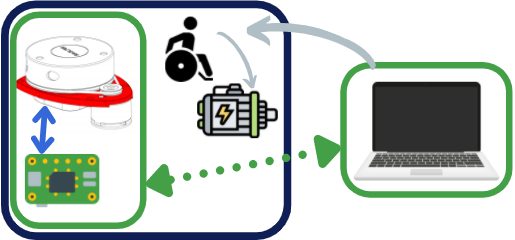
\includegraphics[width=\linewidth]{pics/cart1.png}
        \caption[System representation]{System representation~\cite{ramadhan2021design}}\label{cart1}
    \end{minipage}\hfill
    \begin{minipage}{0.48\textwidth}
        \centering
        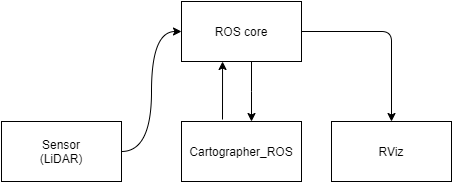
\includegraphics[width=\linewidth]{pics/cart2.png}
        \caption[System data workflow]{System data workflow~\cite{ramadhan2021design}}\label{cart2}
    \end{minipage}\hfill
\end{figure}

\vspace{0.25cm}

\subsubsection{Grid-based FastSLAM (Gmapping)}
GMapping is a highly efficient Rao-Blackwellized particle filter (RBPF) that separates the estimation of the
robot's trajectory hypothesis and the map~\cite{grisetti2007improved}. GMapping effectively builds accurate grid maps
in real-time and is well-suited for indoor environments. The key innovation of Grid-based FastSLAM lies
in its improved proposal distribution that considers both odometry data and the most recent sensor
observations when generating new particles. This approach significantly reduces the number of
particles required for accurate mapping compared to traditional methods that rely solely on odometry
motion models~\cite{1570477}. For medical environments where precise navigation is
crucial, this efficiency is particularly valuable as it enables real-time performance with limited
computational resources. However, the algorithm's performance can be affected in environments 
with limited features or highly symmetric structures, which may require additional sensing modalities or environmental modifications to ensure reliable operation in medical settings.


\newpage

\subsection{Path Planning}
Path planning enables the robot to navigate from a starting
location to a desired goal while avoiding obstacles. Effective path planning algorithms compute feasible and
optimal paths, taking into account the robot's kinematics, dynamics, and the environment's constraints. This section
reviews several key path planning algorithms: Dijkstra's Algorithm, A* Algorithm, Rapidly-exploring Random Trees (RRT),
and the Dynamic Window Approach (DWA).


\subsubsection{Dijkstra's Algorithm}
Dijkstra's algorithm, developed by E. Dijkstra in 1959, represents an approach to solving the single-source shortest path problem in weighted graphs. The algorithm determines the minimum cost path from a source vertex to all other vertices in a graph with non-negative edge weights. For a directed weighted graph \(G = (V,E)\), where \(V\) represents the set of vertices and \(E\) the set of edges, Dijkstra's algorithm maintains a set \(S\) of vertices whose final shortest-path weights from the source have been determined. The algorithm operates by iteratively selecting the vertex \(u \in V - S\) with the 
minimum shortest-path estimate, adding \(u\) to \(S\), and relaxing all edges leaving \(u\). The core evaluation function can be expressed as:

\begin{equation}
    d(v) = \min \{d(u) + w(u,v)\}
\end{equation}

\noindent where \(d(v)\) represents the shortest distance to vertex \(v\), \(d(u)\) is the distance to the current vertex \(u\), and \(w(u,v)\) is the weight of the edge connecting vertices \(u\) and \(v\).



\noindent While Dijkstra's algorithm guarantees finding the optimal path in static 
environments, experimental analysis has shown that it explores significantly more nodes
than informed search methods like A*. As demonstrated in the comparative study
by~\cite{alija2015analysis}, Dijkstra's algorithm exhibits an average search time
approximately 466ms slower than A* in grid-based environments, despite both algorithms
finding paths of identical length.

\newpage

\subsubsection{A* Algorithm}
The A* algorithm represents one of the most efficient heuristic search methods for finding optimal paths in static environments~\cite{gul2019comprehensive}. Its effectiveness stems from combining Dijkstra's algorithm's thoroughness with the added benefit of heuristic estimation. The algorithm employs an evaluation function \(F(n)\) that consists of two components:

\begin{equation}
    F(n) = G(n) + H(n)
\end{equation}

\noindent where \(G(n)\) represents the actual cost from the start node to the current node \(n\), and \(H(n)\) is the heuristic estimated cost from node \(n\) to the goal. The heuristic component \(H(n)\) can be calculated using various distance metrics, as illustrated in Figure~\ref{fig:astar_distances}.

\begin{figure}[H]
    \centering
    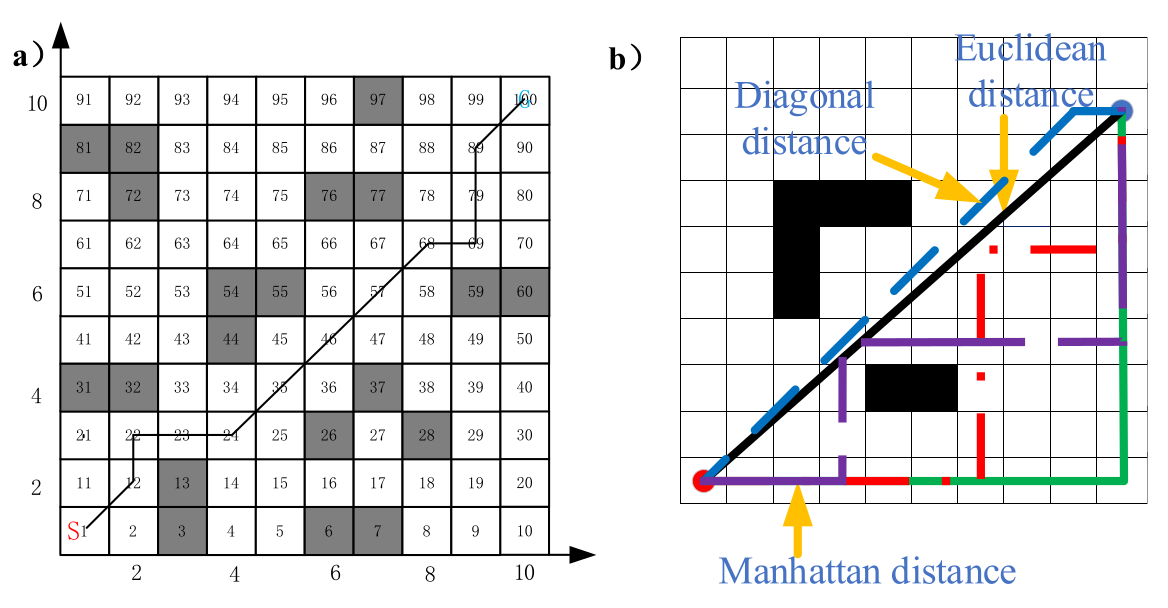
\includegraphics[width=5.5in]{pics/astar_distances.png}
    \caption[Schematic diagram of grid method and paths generated by different distance functions]{(\textbf{a}) Schematic of A* grid (\textbf{b}) Paths from different distance functions~\cite{xiang2022combined}}\label{fig:astar_distances}
\end{figure}

\noindent Recent improvements to the traditional A* algorithm have addressed several key limitations
through three primary enhancements. First, the incorporation of obstacle information into the 
evaluation function improves convergence speed and path quality, modifying the function to:

\begin{equation}
    F(n) = G(n) + H(n) + o(n)
\end{equation}

\noindent where \(o(n)\) represents the obstacle information weight. Second, adaptive directional search has been implemented to reduce unnecessary node expansions by focusing on promising directions based on the target position. Third, path smoothing optimization removes redundant waypoints while maintaining path safety, resulting in approximately 5\% reduction in total path length~\cite{xiang2022combined}.

\newpage

\subsubsection{Rapidly-exploring Random Trees (RRT)}
Rapidly-exploring Random Trees (RRT) is a sampling-based path planning algorithm designed for efficiently searching high-dimensional spaces~\cite{ganesan2024hybrid}. It incrementally builds a space-filling tree by randomly sampling points in the space and connecting them to the nearest node in the tree. The algorithm begins with the initialization step, starting with the initial position of the robot as the root node of the tree. In the sampling loop, a point \(q_{\text{rand}}\) is randomly sampled in the space. The nearest node \(q_{\text{near}}\) in the tree to \(q_{\text{rand}}\) is found, and the algorithm moves from \(q_{\text{near}}\) towards \(q_{\text{rand}}\) by a predetermined step size to get \(q_{\text{new}}\). If the path from \(q_{\text{near}}\) to \(q_{\text{new}}\) is collision-free, \(q_{\text{new}}\) is added to the tree. The process terminates when \(q_{\text{new}}\) is close enough to the goal, allowing for the reconstruction of the path.

\vspace{-0.02cm}

\begin{algorithm}[H]
    \caption{RRT* Framework}\label{alg:rrt}
    \begin{algorithmic}[1]
    \STATE $T \leftarrow (V, E)$
    \FOR{all values of i from 0 to N}
        \STATE $q_{\text{rand}} \leftarrow \text{uniformsample}(i)$
        \STATE $q_{\text{nearest}} \leftarrow \text{nearestneighbors}(T,q_{\text{rand}})$
        \STATE $(\sigma, q_{\text{new}}) \leftarrow \text{steer}(q_{\text{nearest}},q_{\text{rand}})$
        \IF{$\text{obstaclefree}(\sigma)$}
            \STATE $Q_{\text{near}} \leftarrow \text{nearnode}(q_{\text{new}},T)$
            \STATE $(q_{\text{parent}},\sigma_{\text{parent}}) \leftarrow \text{parentupdate}(Q_{\text{near}},q_{\text{nearest}},q_{\text{new}},\sigma)$
            \STATE $T \leftarrow \text{add}(T,q_{\text{parent}},q_{\text{new}},\sigma_{\text{parent}})$
            \STATE $T \leftarrow \text{Rewire}(q_{\text{new}},T,Q_{\text{near}})$
        \ENDIF
    \ENDFOR
    \RETURN $T$
    \end{algorithmic}
\end{algorithm}

\noindent The RRT* algorithm represents a significant advancement in sampling-based path planning, particularly suited for high-dimensional spaces~\cite{karaman2011sampling}. It employs an iterative tree construction process that begins with the robot's initial configuration. The algorithm generates uniform random samples ($q_{\text{rand}}$) across the configuration space and extends the tree by connecting these samples to the nearest existing nodes ($q_{\text{nearest}}$). A key feature of RRT* is its rewiring mechanism, which continuously optimizes the tree structure by checking for potentially shorter paths through new connections.

\noindent Recent improvements to RRT* have addressed its limitations through various sampling strategies. For instance, hybrid sampling approaches combine uniform and non-uniform sampling methods to balance exploration and exploitation~\cite{ganesan2024hybrid}. This hybrid approach has demonstrated superior performance in terms of convergence rate, success rate, and computational efficiency compared to traditional RRT* implementations, achieving up to 76.14\% faster average convergence rates while reducing node exploration by approximately 48.53\%.

\vspace{-0.08cm}

\begin{figure}[H]
    \centering
    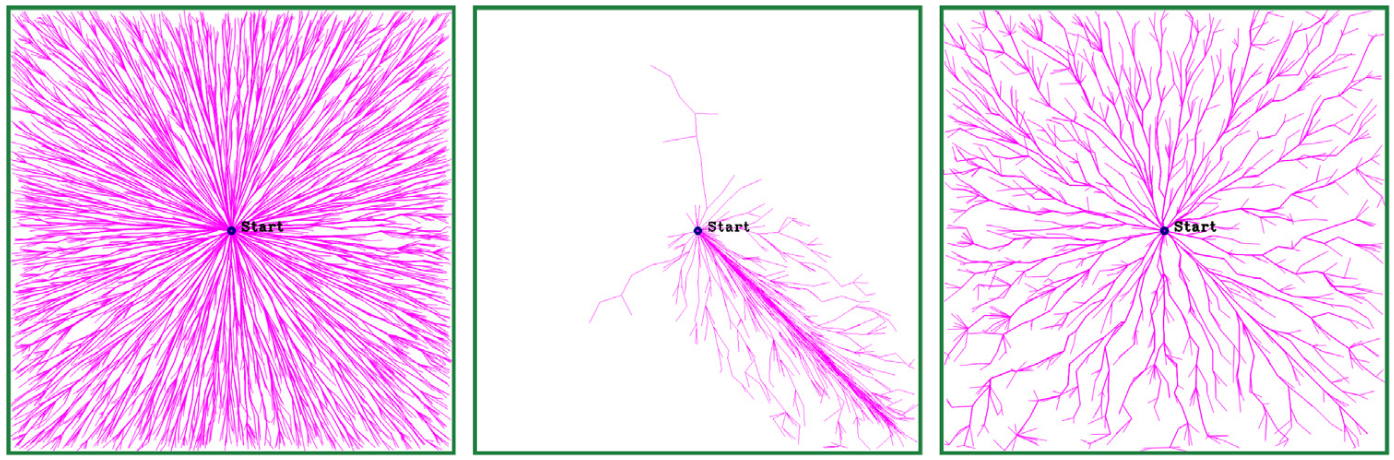
\includegraphics[width=5.2in]{pics/rrt.png}
    \caption[Tree exploration of (\textbf{a}) RRT* and (\textbf{b}) RRT* Connect]{Tree exploration of (\textbf{a}) RRT* and (\textbf{b}) Informed RRT* (\textbf{c}) RRT*-N~\cite{ganesan2024hybrid}}\label{fig:rrt}
\end{figure}

\noindent RRT is efficient in handling high-dimensional and complex spaces and exhibits probabilistic completeness, meaning it will find a solution if one exists given enough time. However, the paths generated may be non-optimal and require smoothing, and the random nature of the algorithm can lead to inconsistent performance. RRT is particularly useful in robotic manipulators and autonomous vehicles where the configuration space is high-dimensional.

\vspace{-0.02cm}

\begin{figure}[H]
    \centering
    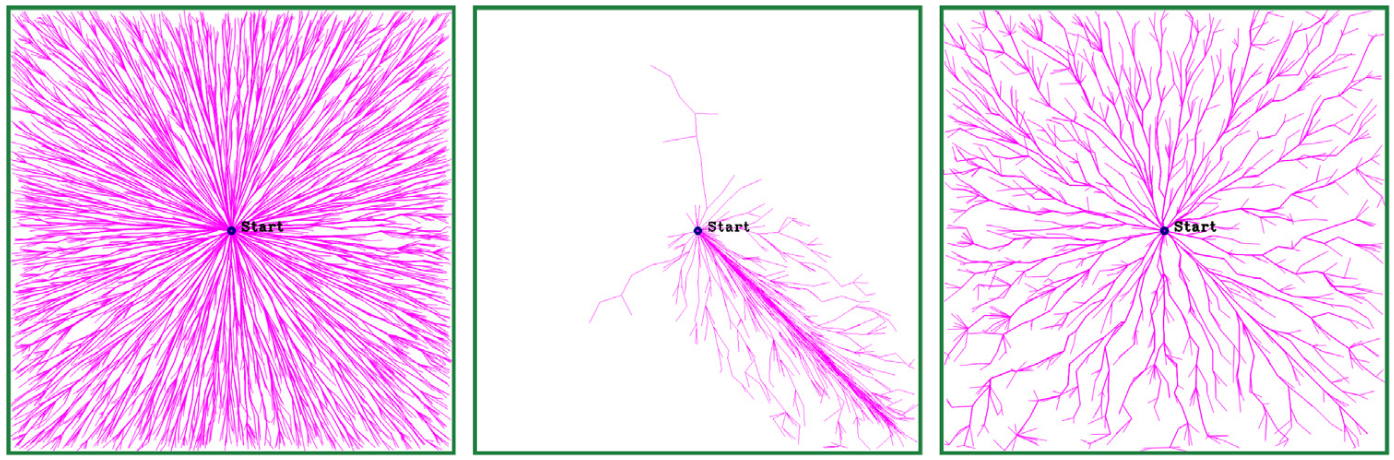
\includegraphics[width=5.2in]{pics/rrt.png}
    \caption[Tree exploration of (\textbf{a}) RRT* and (\textbf{b}) RRT* Connect]{Tree exploration of (\textbf{a}) RRT* and (\textbf{b}) Informed RRT* (\textbf{c}) RRT*-N~\cite{ganesan2024hybrid}}\label{fig:rrt}
\end{figure}


\newpage

\subsubsection{Dynamic Window Approach (DWA)}
The Dynamic Window Approach is a local trajectory planning method that considers
the robot's dynamics to generate feasible and safe motion commands. The algorithm operates by defining
the set of possible velocities considering the robot's current velocity, acceleration limits, and kinematic constraints. A dynamic window limits the velocity space to velocities achievable within a short time frame. For each velocity in the dynamic window, the algorithm simulates the trajectory and evaluates it based on heading (alignment towards the goal), clearance (distance from obstacles), and velocity (preference for higher speeds). The velocity that 
maximizes the objective function, combining the above criteria, is selected. DWA generates motion commands
that are dynamically feasible and allows for real-time obstacle avoidance. However, as a local planner, it may not find a path around large obstacles, suffering from the local minima problem. It requires a good balance between the evaluation criteria. DWA is widely used for real-time navigation in dynamic environments where obstacles may move unpredictably.






\subsection{Robot Operating System 2 (ROS2)}
Since robotic systems involve a combination of many fields in engineering, the task at hand can be complex
and challenging when it comes to integration.
The Robot Operating System 2 (ROS2), formally ROS,  although not an operating system in a traditional sense, is a an open-source framework that provides tools,
libraries, and conventions designed to simplify the task of creating robots.   

\vspace{1.0em}
\begin{figure}[H]
    \centering
    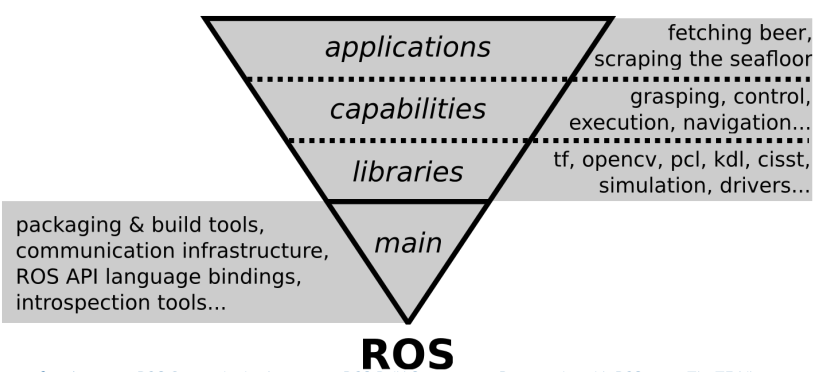
\includegraphics[width=4.8in ]{pics/ree.png}
    \caption[Levels of development with ROS]{Levels of development with ROS~\cite{mosenlechner2012ros}}\label{lt_4}
\end{figure}


\newpage

\subsection{Navigation frameworks in ROS2}
Since robotic applications have different specific requirements, such as indoor or outdoor applications, 3D navigation
with the example of a drone to 2D navigation with the example of a SCARA robot or different optimizations, there are
several frameworks used for robot navigation. Some of the frameworks which are commonly integrated within ROS2 are
explored in this section. 

\subsubsection{Navigation 2 Stacks (Nav2)}
Navigation2~\cite{thomas2014nextgenros}\cite{macenski2020marathon2} is a navigation framework specifically designed for ROS2~\cite{thomas2014nextgenros}, which was built as an improvement on
the previous ROS Navigation~\cite{quigley2009ros} for ROS~\cite{mardereppstein2010office}. It provides a flexible and modular framework for autonomous
navigation~\cite{macenski2020marathon2}. It features behavior trees~\cite{abiyev2016robot} for task execution, a plugin-based architecture
for custom planners and controllers, improved performance leveraging ROS2`s real-time capabilities, and 
costmaps for planning and obstacle avoidance. Nav2 supports various navigation algorithms, making it easier to implement 
techniques like SLAM (Simultaneous Localization and Mapping) and AMCL (Adaptive Monte Carlo Localization). Nav2 
integrates A* and Dijkstra's Algorithm in the global planner to compute optimal paths on a costmap grid, allowing
for the customization of planners as per requirements. For example,  the Dynamic Window Approach (DWA) can
be used in the local planner to compute velocity commands that are safe and feasible, considering the robot's
dynamic constraints and real-time sensor data. Nav2’s flexibility, modularity, and real-time capabilities make
it suitable for a wide range of robots.


\vspace{0.7em}
\begin{figure}[H]
    \centering
    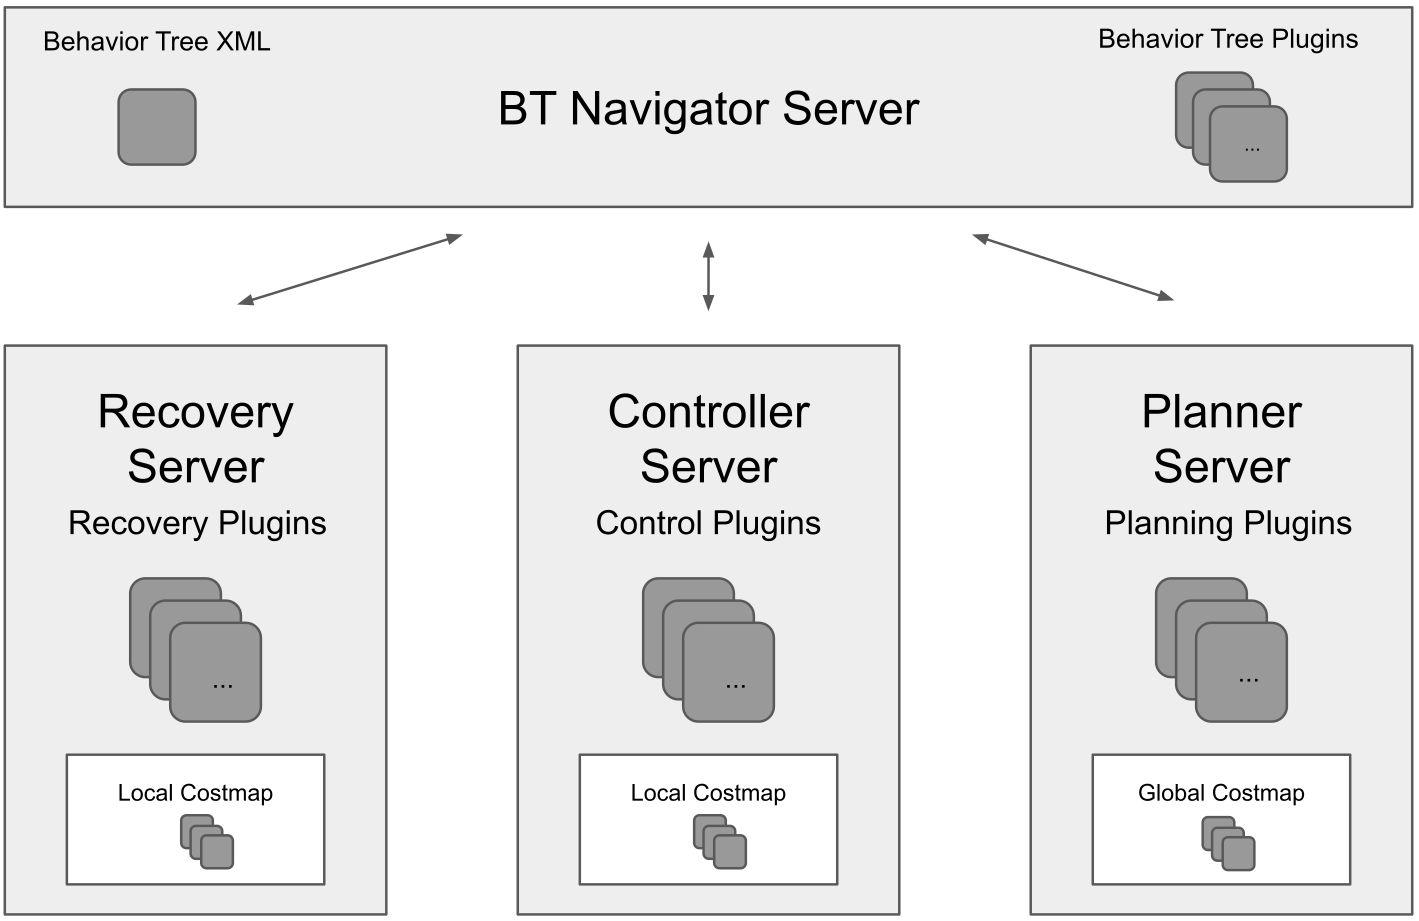
\includegraphics[width=4.5in ]{pics/nav2.png}
    \caption[Overview of Navigation2 design]{Overviewof Navigation2 design~\cite{macenski2020marathon2}}\label{nav2}
\end{figure}


\subsubsection{ARC Nav Stack}
Since most of the existing navigation stacks implemented on ROS and its successor ROS2 are primarily designed for 2D navigation
environments, the approach simplifies computations but it is only suitable for wheeled robots navigating on flat surfaces. There
are serious limitations when dealing with robots that operate in three-dimensional (3D) environments, such as aerial drones or legged
robots traversing uneven terrain. The ARC Nav Stack was introduced~\cite{vishwas2021arc} to overcome this limitation. ARC Nav
utilizes a volumetric representation of the robot's workspace, thus enabling full 3D motion planning and control. ARC Nav uses the OctoMap~\cite{hornung2013octomap}
library for mapping, that represents 3D space using an octree data structure. OctoMap allows for the probabilistic
representation of occupancy, handling sensor noise and uncertainties effectively. The use of an octree structure enables
the compression of the map by recursively combining neighboring voxels with similar information, reducing memory
consumption while maintaining essential details of the environment. ARC Nav is crucial for safe navigation and exploration tasks~\cite{vishwas2021arc}.


\vspace{0.7em}
\begin{figure}[H]
    \centering
    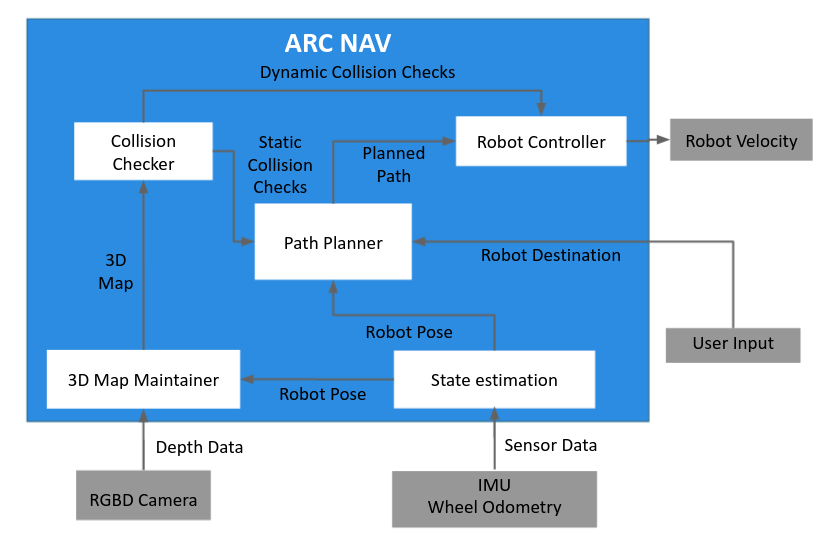
\includegraphics[width=4.0in ]{pics/arc_nav.png}
    \caption[Overview of the ARC Nav Stack Architecture]{Overview of the ARC Nav Stack Architecture~\cite{vishwas2021arc}}\label{arc4}
\end{figure}




\noindent In terms of motion planning, ARC Nav introduces a novel sampling-based algorithm called 2BIT*, which extends the Batch Informed
Trees (BIT*) algorithm~\cite{gammell2015bit} by incorporating a bidirectional search approach. Traditional BIT* combines features
from algorithms like Fast Marching Tree (FMT*) and Informed RRT*, focusing on efficiency and optimality in path planning. The 2BIT* algorithm
enhances BIT* by growing two trees simultaneously: one rooted at the start position and the other at the goal position. These trees expand towards each other, aiming to find a connection that results in a feasible path.

\noindent A key innovation in 2BIT* is the introduction of strategy switching during the connection attempts between the two trees.
Two primary strategies are employed: connecting the most recently added node of one tree to the nearest node in the other
tree, and connecting it to a randomly chosen node. By allocating probabilities to each strategy and switching between them
based on certain conditions, the algorithm adapts to the planning scenario, reducing the time taken to find an initial
path and improving convergence towards the shortest possible path. This adaptive approach addresses the 
limitations observed in algorithms like RRT-Connect~\cite{Kuffner2000RRTconnectAE}, which, while efficient in finding initial
paths, do not guarantee asymptotic optimality and lack strategy variability. 
The architecture of ARC Nav is modular, similar to Nav2, allowing for easy customization of components like state estimation,
mapping, planning, and control. 



\subsubsection{RTAB-Map}

A 2D lidar sensor mounted at a fixed height may fail to detect overhanging obstacles like tables and chairs
or low-lying objects such as trash cans, leading to incomplete maps and potential navigation failures.To address these challenges~\cite{labbe2018rtabmap} explored the use of RTAB-Map (Real-Time Appearance-Based Mapping), a graph-based SLAM approach that integrates
data from multiple sensors to generate comprehensive 3D maps. By fusing information from an RGB-D camera, a 2D lidar, an IMU, and wheel odometry, the robot can construct a more accurate representation of its environment, enhancing navigation and obstacle avoidance capabilities.



\vspace{0.7em}
\begin{figure}[H]
    \centering
    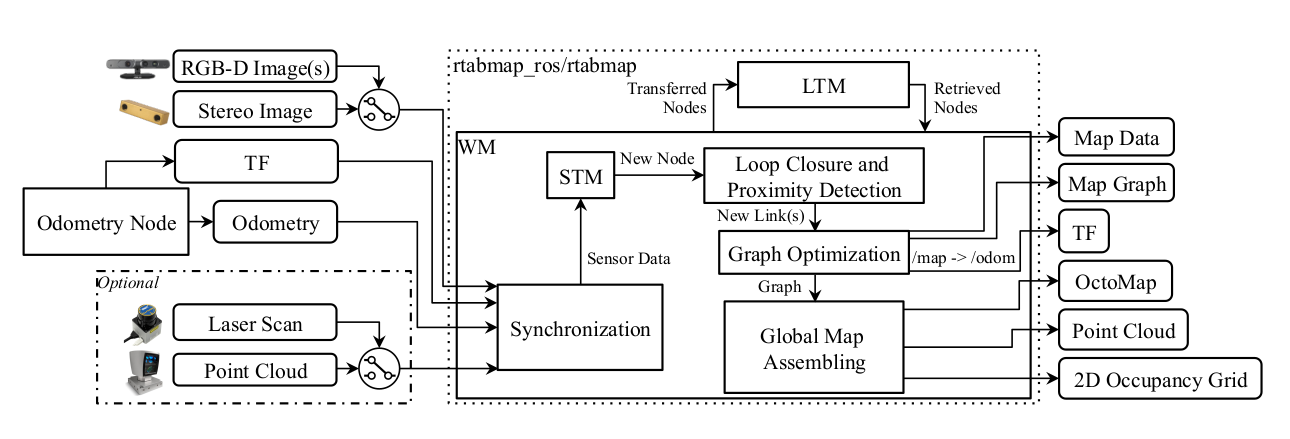
\includegraphics[width=6.3in, height=3.2in]{pics/rtab1.png}
    \caption[Schematic flowchart of RTAB-Map]{Schematic flowchart of RTAB-Map~\cite{labbe2018rtabmap}}\label{rtab_flow}
\end{figure}



\subsubsection{Micro-ROS}
Mobile robots are becoming more complex and integrating microcontrollers into their architectures is 
essential for modularity and efficient
resource management. Micro-ROS is designed for microcontrollers and embedded systems thus it can integrate 
them with ROS2. In~\cite{nguyen2022microros}, MicroROS
was evaluated on the quality of service (QoS) and communication capabilities. Micro-ROS is optimized for 
low memory usage and efficient
processing, it utilizes a lightweight communication protocol called DDS for Extremely Resource Constrained 
Environments (DDS-XRCE)~\cite{nguyen2022microros},
which allows micro-ROS clients on microcontrollers to communicate efficiently with teh micro-ROS agent. 
The micro-ROS agent, running on a more powerful processor, acts as a bridge between the micro-ROS client 
and the ROS 2 network, translating communication between DDS-XRCE and the standard DDS protocol used by 
ROS 2 nodes.


\vspace{0.7em}
\begin{figure}[H]
    \centering
    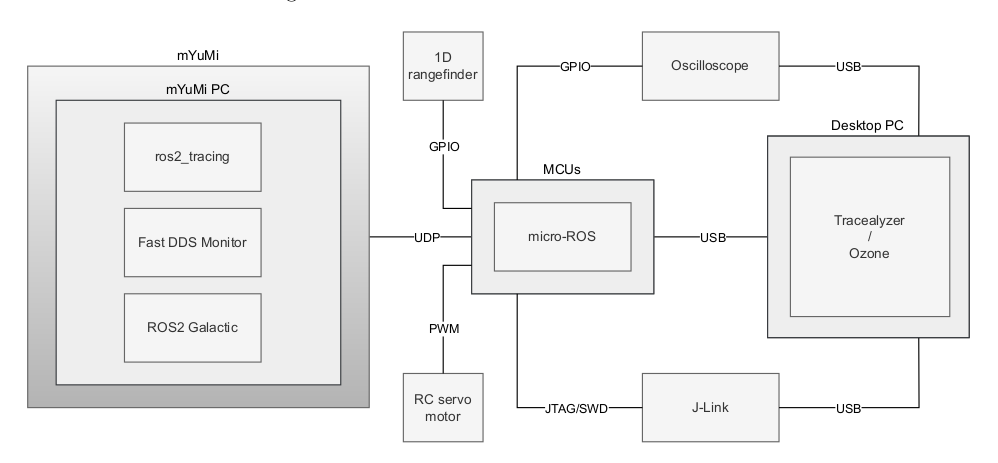
\includegraphics[width=6.4in ]{pics/microROS.png}
    \caption[Micro-ROS connecting mYuMi robot to MCUs]{Micro-ROS connecting mYuMi robot to MCUs~\cite{nguyen2022microros}}\label{microros}
\end{figure}



\subsubsection{Autoware-Based Navigation}
Autoware is an open-source software stack specifically designed for autonomous driving applications, providing an extensive
range of functionalities required for self-driving vehicles, including perception, localization, planning, and control. 
Built on top of ROS 2, Autoware integrates data from various sensors such as lidars, cameras, GPS, and IMUs to perceive the 
environment and accurately localize the vehicle within it. The framework employs advanced algorithms for object detection, 
lane recognition, and obstacle avoidance, enabling vehicles to navigate complex urban environments.

\noindent Autoware`s modular and adaptable design allows developers to tailor the system to specific vehicles and 
operational
requirements. An integral part of this ecosystem is Autoware
Perf, a tracing and performance analysis framework developed to evaluate and optimize the performance of ROS 2 applications
within Autoware. AutowarePerf extends existing tracing tools, such as ROS 2 Tracing and LTTng, to measure execution times 
of nodes and inter-node communication latencies. This framework enables developers to gain insights into the system's 
end-to-end latency, identify bottlenecks, and optimize performance to meet real-time constraints essential for autonomous vehicles.
By providing detailed performance metrics and visualization tools, Autoware Perf facilitates the development of 
high-performance, reliable autonomous driving systems. It addresses challenges such as selective measurement of specific nodes, 
insertion of trace points for communication latency measurement, and overall latency calculation across the system. 
Through these capabilities, Autoware and its associated tools contribute significantly to the advancement of autonomous vehicle 
technologies, emphasizing safety, efficiency, and scalability.\\

\vspace{0.005in}

\subsubsection{Comparison of ROS2 Navigation Frameworks}

\begin{table}[h]
    \centering
    \renewcommand{\arraystretch}{2.0}
    \setlength{\tabcolsep}{4.4pt}
    \footnotesize
    \begin{tabular}{|p{2.4cm}|p{2.2cm}|p{2.95cm}|p{1.9cm}|p{4.7cm}|}
      \hline
      \rowcolor[gray]{0.8} 
      \textbf{Framework} & \textbf{\makecell[{{l}}]{Dimensions\\Supported}} & \textbf{Primary Sensors} & \textbf{Complexity} & \textbf{Ideal Applications} \\
      \hline
      Nav2 & 2D & LIDAR, 2D Sensors, Odometry & Medium & Indoor ground mobile robots on flat surfaces\\
      \hline
      ARC Nav & 3D & Depth Cameras, 3D LIDAR & High & Drones, underwater vehicles, multi-level navigation\\
      \hline
      RTAB-Map & 3D & RGB-D and Stereo Cameras, LIDAR & High & 3D mapping (High-precision), exploration \\
      \hline
      Cartographer & 2D and 3D & Lidar, IMU & High & Real-time SLAM, indoor (High-precision) mapping \\
      \hline
      Hector SLAM & 2D & LIDAR & Medium & Fast mapping without odometry, indoor navigation \\
      \hline
      Gmapping & 2D & LIDAR, Odometry & Medium & Indoor SLAM with wheel odometry \\
      \hline
      Micro-ROS & 2D (primarily) & \makecell[{{l}}]{\raisebox{-1.5pt}{Various embedded}\\sensors} & Low & Resource-constrained devices \\
      \hline
      Autoware-Based Navigation & 3D & LIDAR, GPS, IMU, Camera & High & Autonomous driving \\
      \hline
    \end{tabular}
    \caption{Comparison of ROS2 Navigation Frameworks}\label{tab:comparison_ros2_navigation_frameworkss}
\end{table}


\newpage
\subsection{Related Works}
\subsubsection{Navigation with Gmapping and AMCL}
\noindent In~\cite{kok2020intelligent}, a medical robot which uses ROS was implemented for assistance and conveyance of incoming patients in a hospital. The shortest distance algorithm approach
was was utilized, while the Grid-based mapping (Gmapping) is employed to map the environment. Gazebo and Rviz are visualization tools which were
also used in this research. For patient-staff communication, a voice recognition system that integrates with ROS firmware mapping algorithm is done. On the user interface design, the user
can communicate with the robot and even see the locations where robot can go~\cite{kok2020intelligent}. The Policlinic in visualized in
RviZ tool as can be seen in the \figref{lt_1} below. The robot uses the Adaptive Monte Carlo Localization (AMCL)~\cite{chung2022improved} algorithm for localization and that combined
with the mapping algorithm achieves what is known as Simultaneous Localization and Mapping (SLAM). 


\begin{figure}[H]
    \centering
    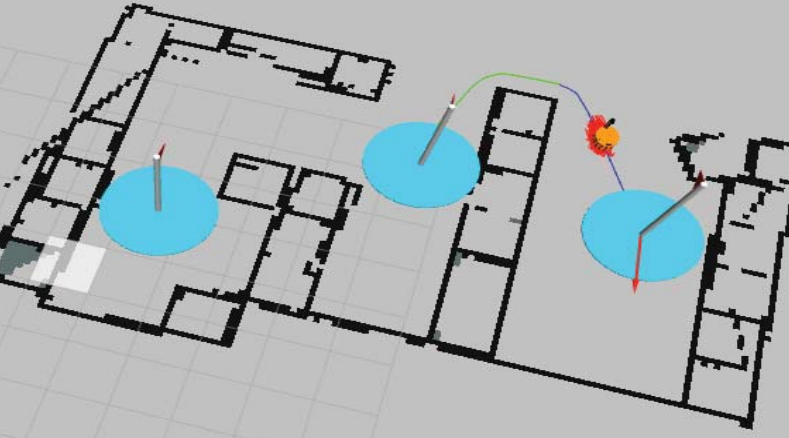
\includegraphics[width=3.2in]{pics/lt_1.png}
    \caption[Localization of the Policlinic in Rviz simulation tool]{Localization of the Policlinic in Rviz simulation tool~\cite{kok2020intelligent}}\label{lt_1}
\end{figure}

\begin{figure}[H]
    \centering
    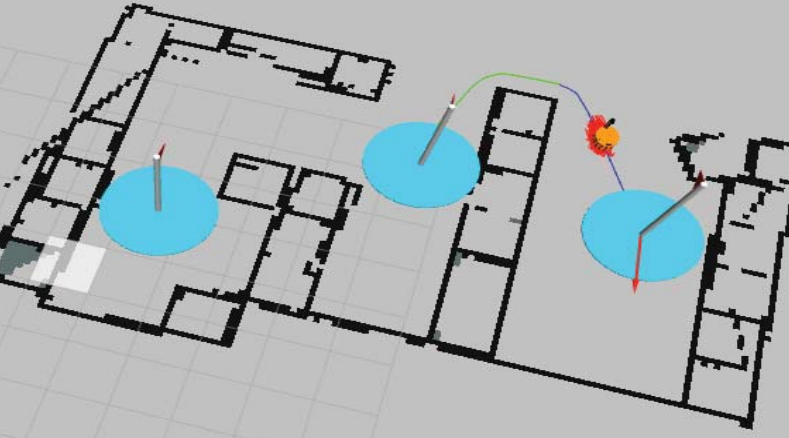
\includegraphics[width=3.2in]{pics/lt_1.png}
    \caption[Localization of the Policlinic in Rviz simulation tool]{Localization of the Policlinic in Rviz simulation tool~\cite{kok2020intelligent}}\label{lt_1}
\end{figure}

\subsubsection{Navigation with RGB-D}
\noindent Another relevant study focuses on positioning and navigation of a medical robot by the use of
RGB-D cameras. These cameras provide color and depth information of an image hence are more accurate and 
very suitable for environmental mapping. This approach supercedes the traditional SLAM algorithms by 
enhancing feature point extraction and mismatch elimination using Random Sample Consensus (RANSAC), thus resulting in better robot
navigation accuracy. The image and depth information data from the RGB-D camera can also be stitched together
with the results from pose estimation to generate a 3D point cloud as shown in \figref{pcl_stitch}.
The research also shows the reduction on the impact of lighting and environmental changes
on navigation accuracy~\cite{jia2023rgbd}. Despite the improvements, RGB-D cameras still struggle with heavy computational
requirements and delays in case of real-time processing. There is also a high similarity between day and 
night in most hospital corridors, significant changes in light intensity between day and night which make
the problem even more challenging. This might be very critical especially considering
in a hospital where urgency is important. Future researchers are working on integrating deep learning and
artificial intelligence to achieve deeper optimization of RGB-D  visual based SLAM\cite{makhubela2023vslam}.


\begin{figure}[H]
    \centering
    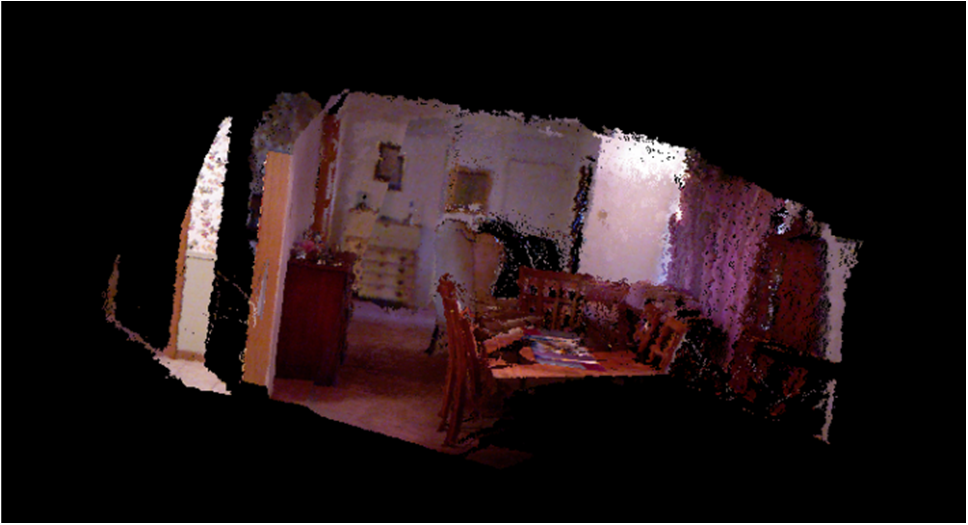
\includegraphics[width=3.2in ]{pics/pcl_stitch.png}
    \caption[Point cloud stitching map]{Point cloud stitching map~\cite{makhubela2023vslam}}\label{pcl_stitch}
\end{figure}

\noindent The study on the ROM20, an autonomous mobile robot platform for medical purposes, demonstrates
the use of modular designs and omni-directional movement through mecanum wheels~\cite{baskoro2020autonomous}.
The ROM20 can be equipped
with various subsystems, such as disinfectant sprayers, UVC lamps, and food delivery modules as demonstrated in \figref{bask}, hence it is versatile
for different medical tasks. However, mecanum wheels can be complex to control and lack in perfomance,
particularly on uneven or cluttered floors. This robot also only uses Bluetooth via a Teensy 4.0 microcontroller
making it limited to a short-range of 22 meters. In essence, ROM20 is not a fully autonomous robot, a 
lot of improvements can be made. 


\begin{figure}[H]
    \centering
    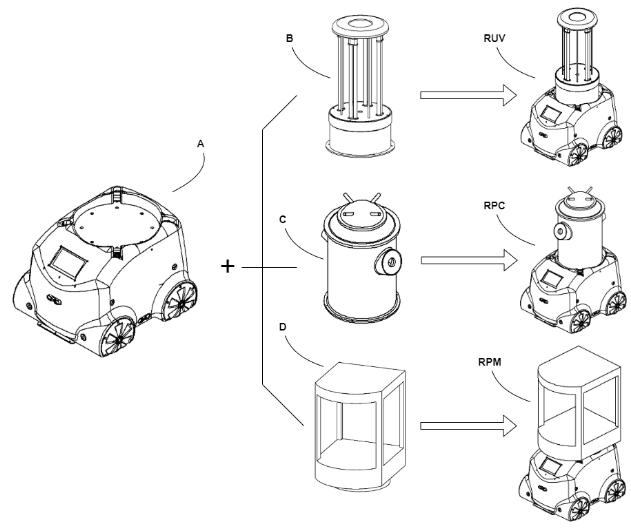
\includegraphics[width=3.8in ]{pics/modular_rom20.png}
    \caption[Modular sybsystems of ROM20]{Modular subsystems of ROM20~\cite{baskoro2020autonomous}}\label{bask}
\end{figure}

\subsubsection{Navigation with Hector SLAM and AMCL}
\noindent While still on the omnidirectional robots, ARIS 1.0 is an autonomous multitasking medicals service
robot that can be used in hospitals, particularly during pandemics~\cite{dunuwila2024aris}. ARIS 1.0 is equipped with a three-wheeled
omnidirectional mobile platform as shown in \figref{ar_1}, achieving three Degrees of Freedom (DOF) neck mechanism, and ROS-based
semi-autonomous navigation capabilities. It's unique features include a telepresence system, IoT-based
vital sign extraction, and the ability to communicate in regional languages, specifically Sinhala. The architecture of this robot was based on three parts; sensors, controllers, and Actuators. The main sensors were the 2D LiDAR, Camera, wheel encoders and a microphone. Three controllers were used; Jetson Nano for High level control which processed the sensor data and integrated it with how the display and speaker would 
function in the actuators part. The low level controllers are the Arduino Mega which controls the encoders and the motor controllers, 
and the Raspberry Pi 3B+ for Limit switches and mainly control the neck mechanism for the robot. As for navigation, Hector SLAM~\cite{nagla2020hector} is used for mapping and Adaptive Monte Carlo Localization (AMCL)~\cite{chung2022improved} is
applied for localization.
The robot was able to facilitate remote ward rounds and telemedicine. However, the ARIS 1.0 system's reliance on a
single 2D LiDAR for navigation poses challenges in case of a dynamic hospital setting which can have a complex
environment, since its precision is limited. 



\vspace{1.5em}

\begin{figure}[H]
    \centering
    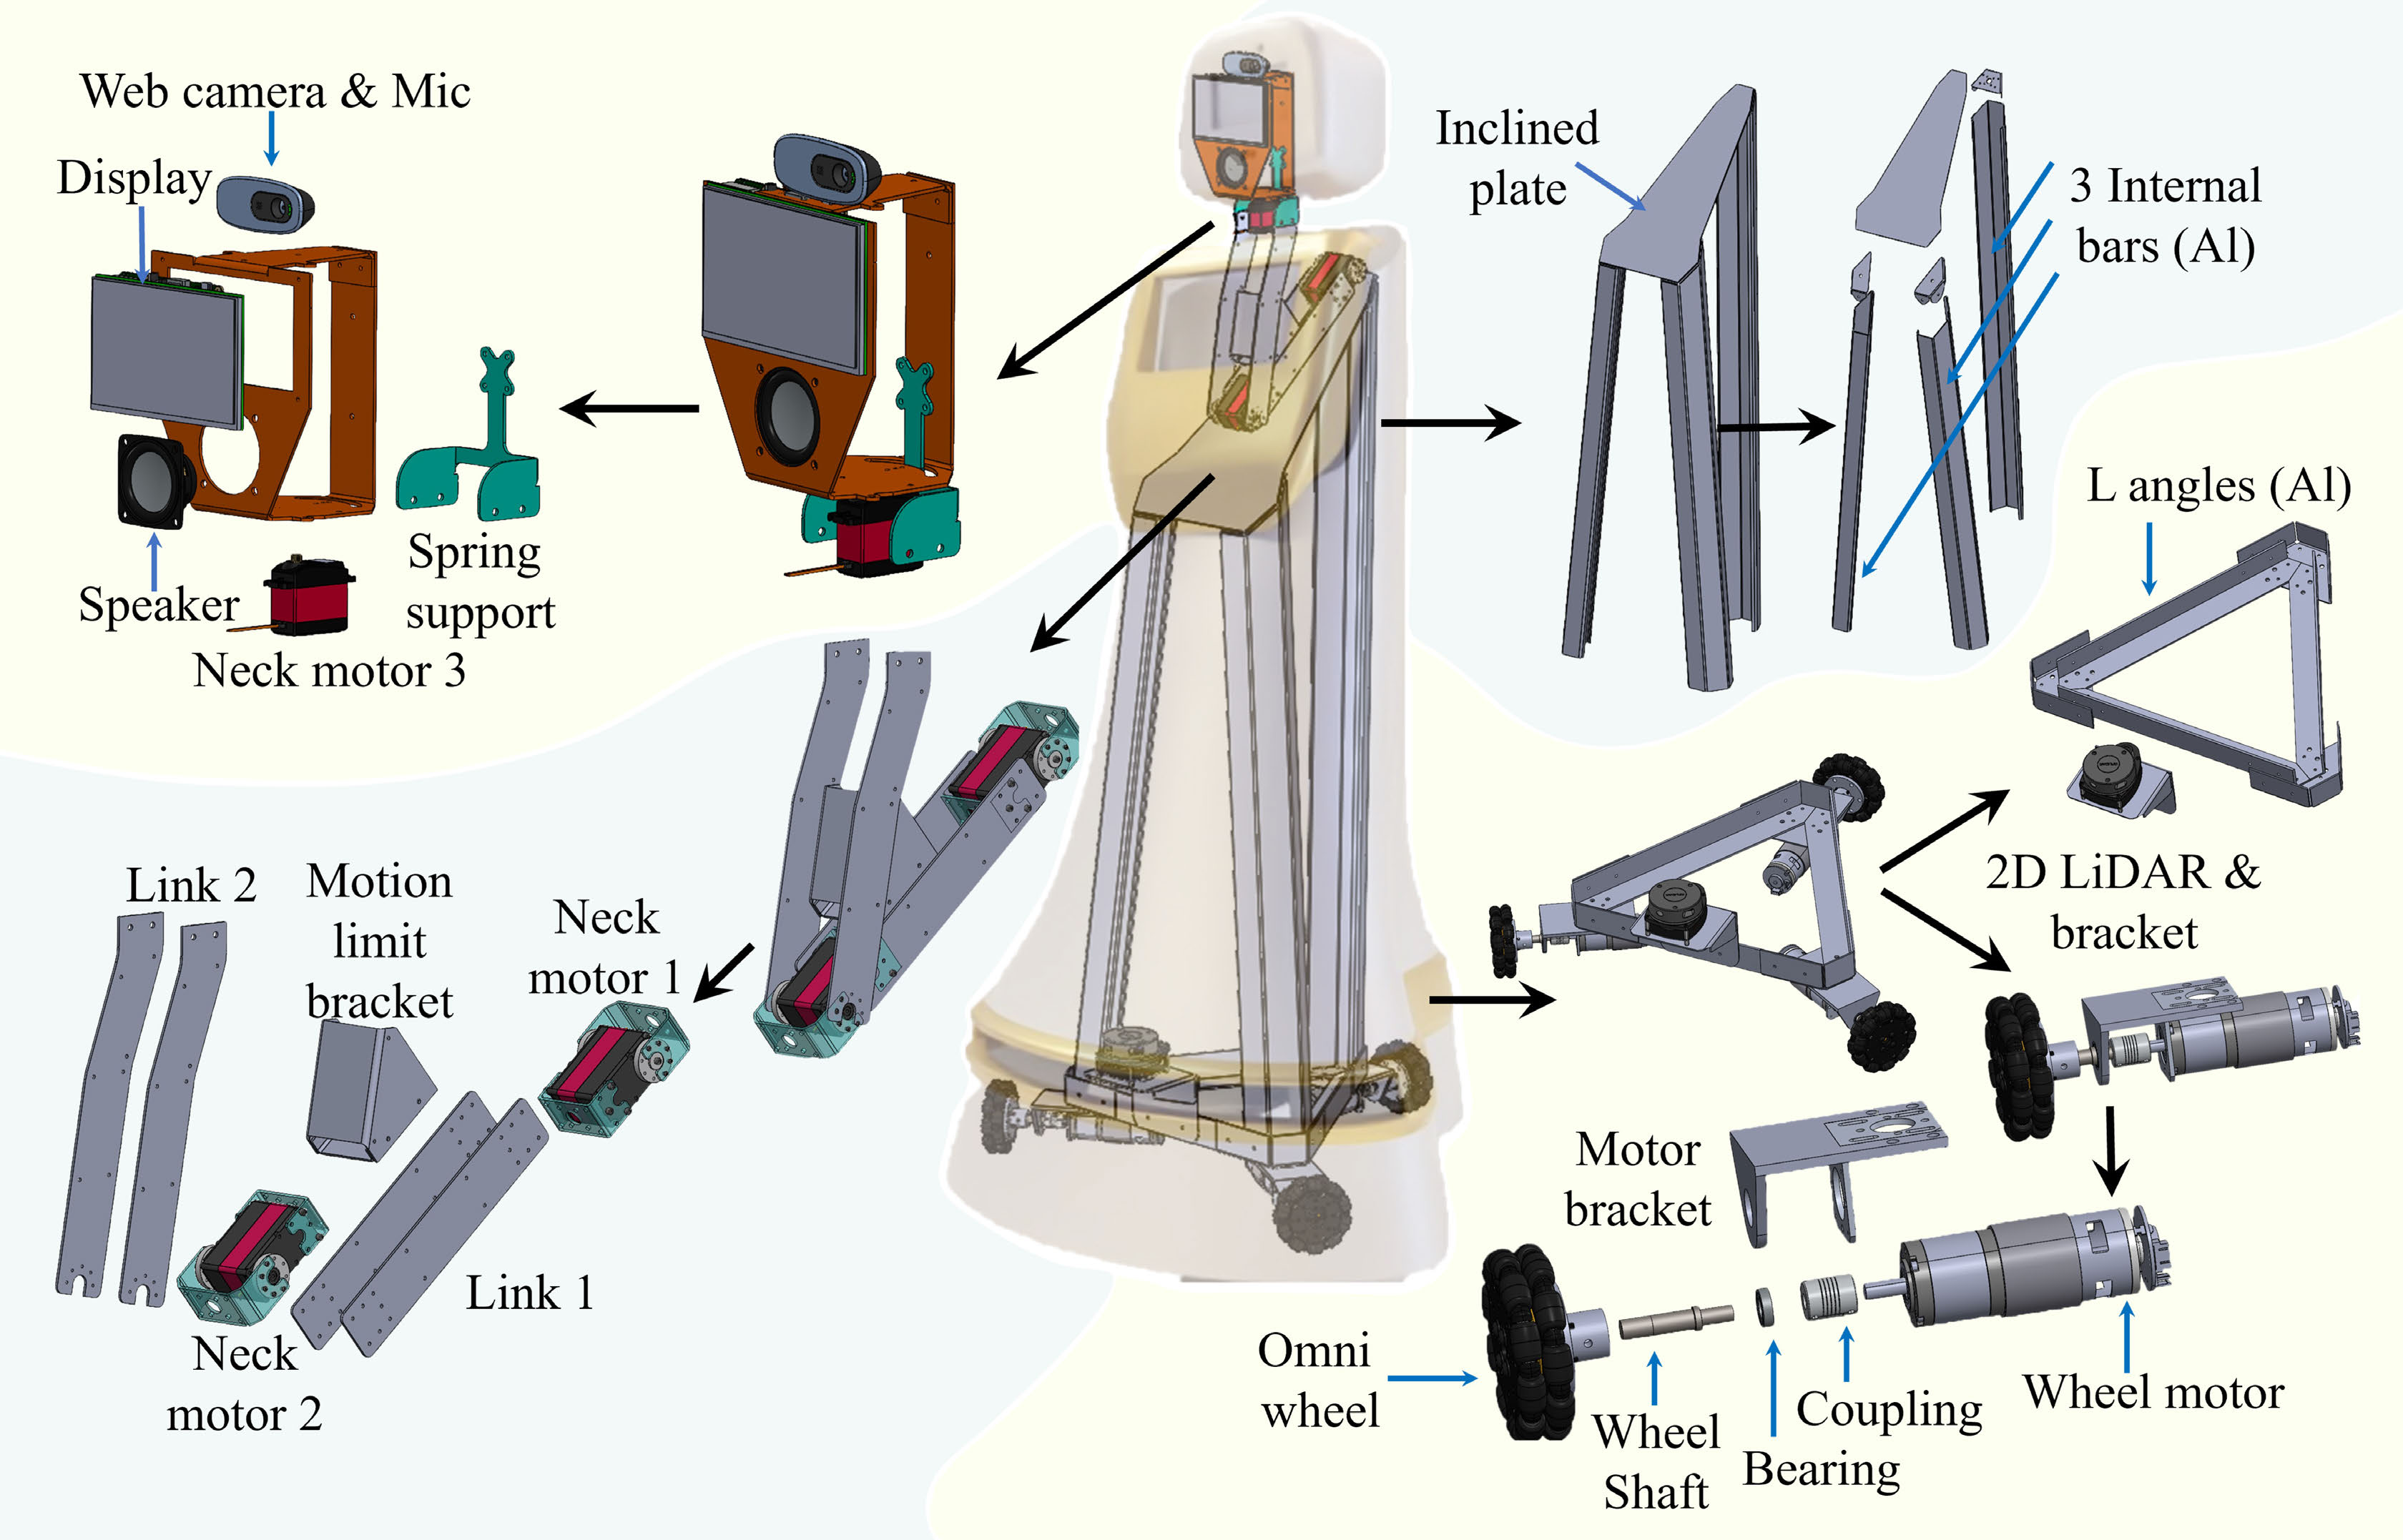
\includegraphics[width=5.5in ]{pics/explod_aris.png}
    \caption[Exploded view of ARIS 1.0]{Exploded view of ARIS 1.0~\cite{nagla2020hector}}\label{ar_1}
\end{figure}

\noindent Moreover, the study in~\cite{valner2022scalable} explores the use of autonomous robots to transport time-critical samples, such as
blood samples, from the Intensive Care Unit (ICU) to the laboratory in Tartu University Hospital. The robot's objective is to automate
non-medical task, such as transporting medical items, to free healthcare professionals from secondary duties, thus allowing more time focus
on patient care. The robot's were deployed using Robotics Middleware Framework (RMF)~\cite{quigley2020ros2}, an open-source fleet management
platform designed for coordinating and integrating fleets of robots within an existing building infrastructure like doors and elevators. 

\vspace{1.0em}
\begin{figure}[H]
    \centering
    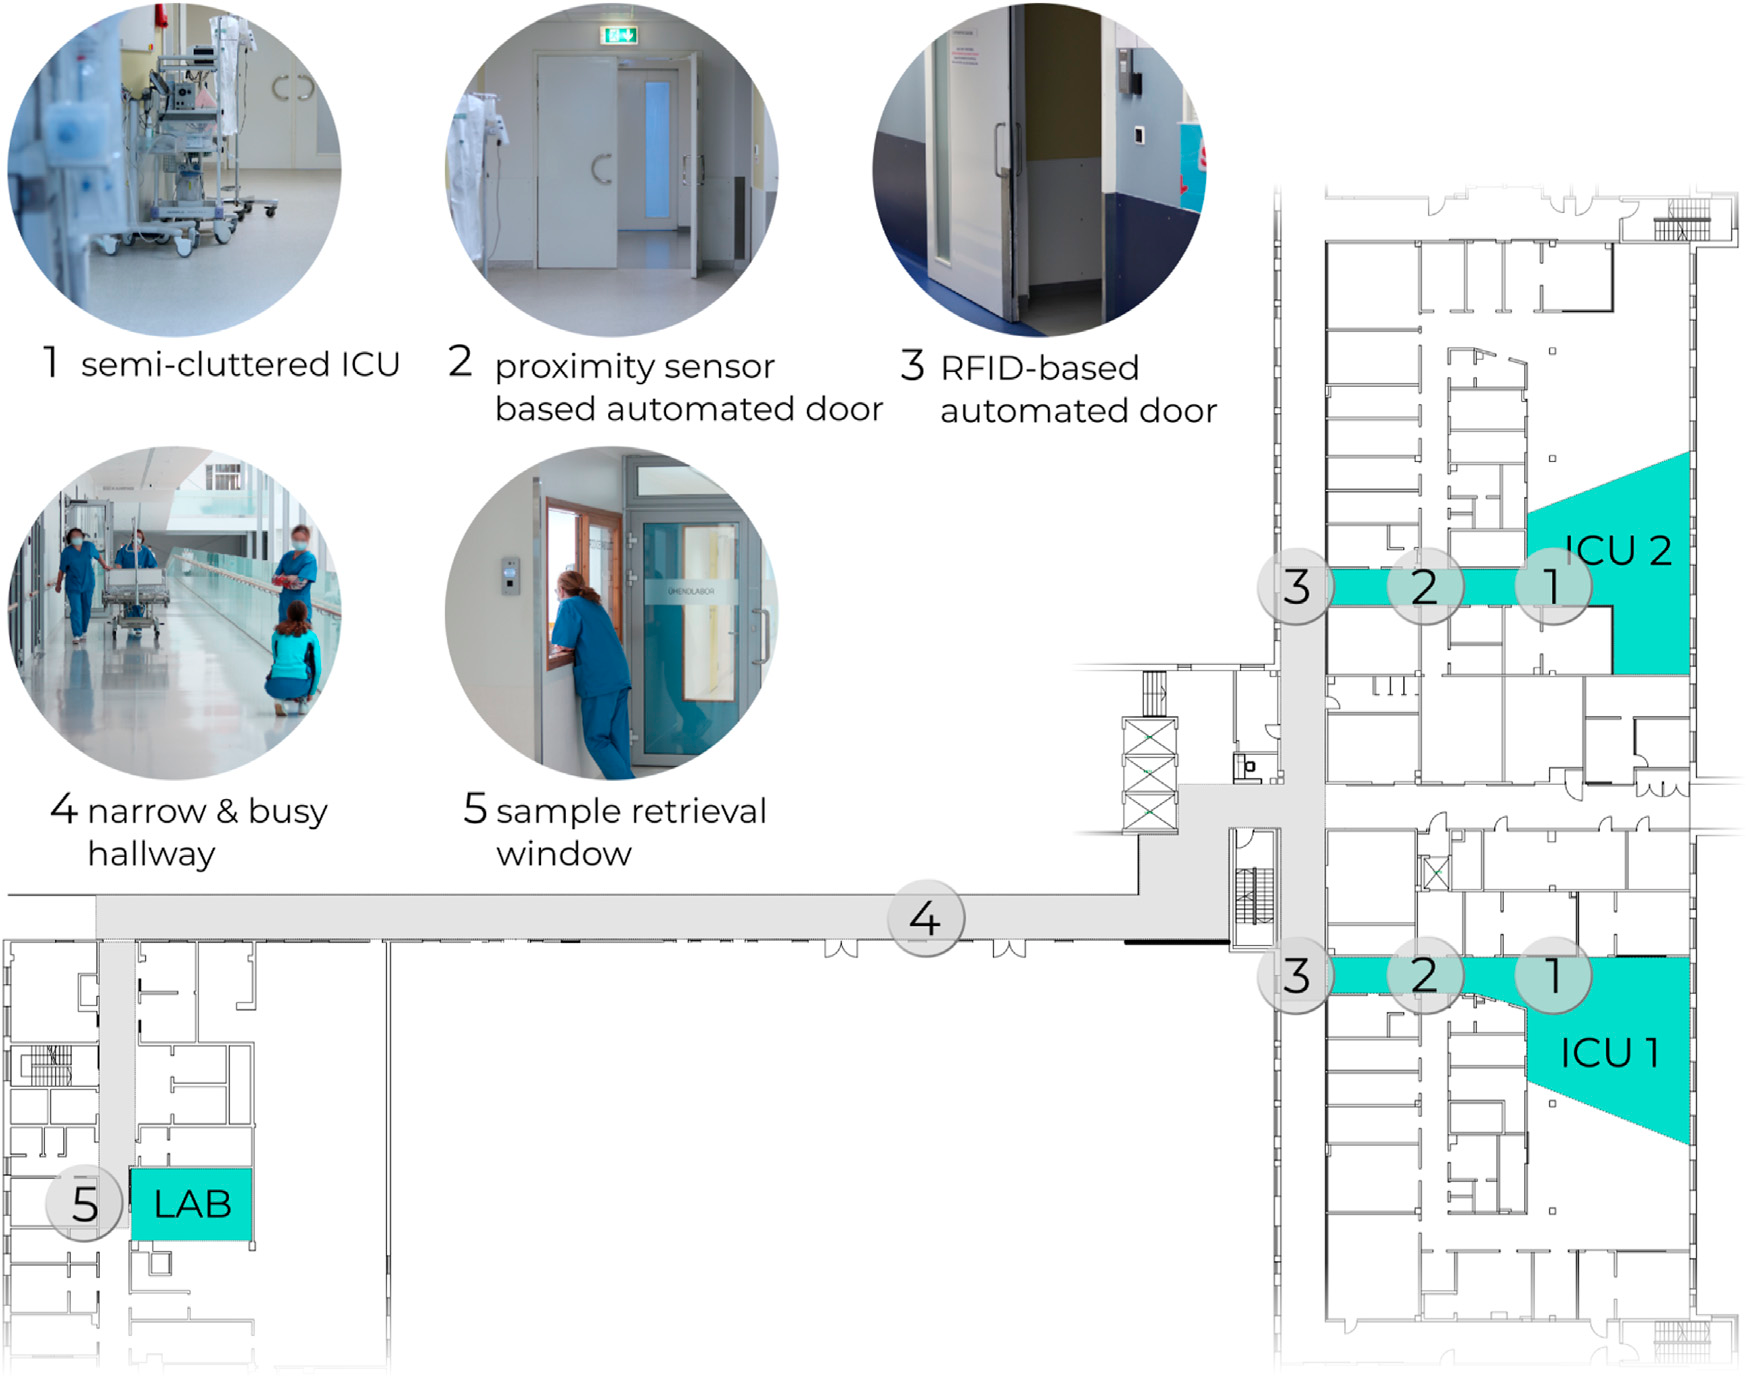
\includegraphics[width=5.5in]{pics/floor_tarta.png}
    \caption[Floorplan of Tarta University Hospital during object transportation]{Floorplan of Tarta University Hospital during object transportation~\cite{valner2022scalable}}\label{tarta1}
\end{figure} 

\vspace{-0.1em}

\noindent The use of RMF allowed for real-time task distribution, route planning, and system monitoring of the robots. RMF system was built as a
distributed application using ROS2 nodes. The nodes communicate through ROS2 topics and services, and the Data Distribution Service (DDS) protocol
allows real-time communication between the robots and the RMF system. Most importantly, navigation commands and robot status are sent via topics and
services.\@ Since RMF has the hospital infrastructure, custom ROS2 nodes were developed to control door mechanisms via commands received from the RMF.\@
An example is given where a ROS2 node running on a Raspberry Pi is connected to the door controllers and activated the servo motors that
opened the doors upon receiving commands from the RMF.\@ 


\begin{figure}[H]
    \centering
    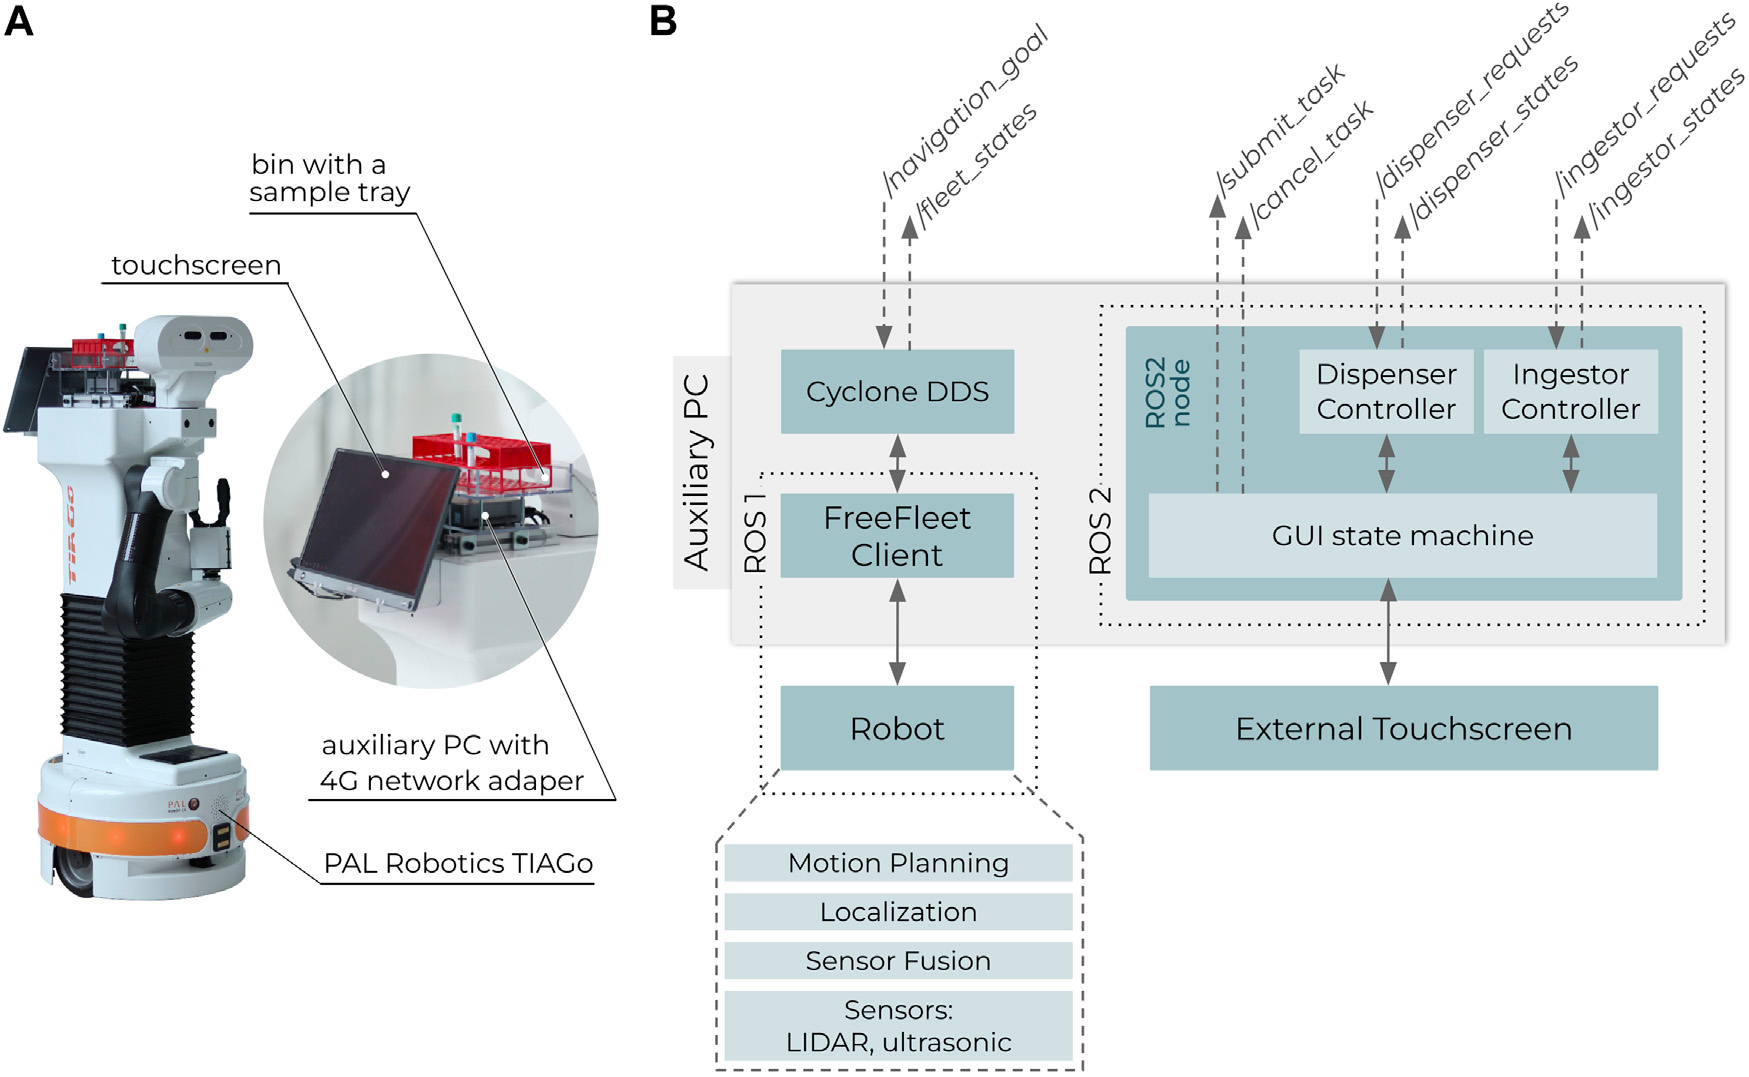
\includegraphics[width=4.5in]{pics/rmf2.png}
    \caption[PAL Robotics TIAGo hardware \textbf{(A)}. Software setup of the whole robot \textbf{(B)}.]{PAL Robotics TIAGo hardware \textbf{(A)}. Software setup of the whole robot \textbf{(B)}.~\cite{valner2022scalable}}\label{stm32_pi}
\end{figure}





\subsection{Summary of the literature review}
The literature emphasizes that effective robot navigation hinges on four key components: perception, localization, cognition, and motion control. Perception involves acquiring environmental data through sensors such as cameras, LiDAR, and ultrasonic sensors. Localization determines the robot's position within the environment, while cognition focuses on path planning and obstacle avoidance decision-making processes. Motion control translates these decisions into motor commands to execute navigation tasks.
Various localization and mapping techniques have been explored to enhance navigation accuracy. Dead reckoning provides position estimates based on previous movements but is prone to cumulative errors. Kalman Filters (KF) and Extended Kalman Filters (EKF) offer probabilistic approaches for state estimation and handling of linear and nonlinear systems. However, they require accurate models and may need to cope better with complex environments. Particle Filters, such as Monte Carlo Localization (MCL) and its adaptive variant AMCL, represent the robot's belief state with weighted particles, accommodating non-linearities and non-Gaussian noise, making them suitable for dynamic settings.
Algorithms like Grid-based FastSLAM (Gmapping) and Hector SLAM are used for mapping. Gmapping builds occupancy grid maps in real-time, which is ideal for indoor environments. At the same time, Hector SLAM relies on high-frequency LiDAR data without requiring odometry, which is beneficial for robots lacking wheel encoders.
Path planning algorithms are crucial for safe and efficient navigation. The A* algorithm, an enhancement of Dijkstra's algorithm, introduces heuristics to expedite the search for optimal paths, balancing efficiency and computational demands. The Dynamic Window Approach (DWA) serves as a local planner, generating feasible velocity commands by considering the robot's dynamics, which is essential for navigating dynamic environments like hospital corridors.
The Robot Operating System 2 (ROS2) and its Navigation 2 Stack (Nav2) provide a robust framework for integrating these algorithms. Nav2's modular architecture allows for customization and seamless incorporation of various navigation strategies, leveraging ROS2's enhanced communication and real-time capabilities. Alternative frameworks like ARC Nav and RTAB-Map offer extended functionalities but may be unnecessarily complex or resource-intensive for ground-based robots in structured environments.
Considering related works, robots employing Gmapping and AMCL have demonstrated reliable navigation in hospital settings, with additional studies highlighting the benefits of sensor fusion using devices like RGB-D cameras for improved environmental perception. However, computational efficiency remains a concern, especially for real-time applications on resource-limited hardware.

\subsubsection*{Selection of Algorithms for the Project}

Based on the literature and the project objectives—developing an autonomous robot for medicine dispensing in hospital wards—the following algorithms have been selected:

\noindent\textbf{Localization and Mapping:} 
\begin{itemize}
    \item Adaptive Monte Carlo Localization (AMCL) \\
    \textit{Justification:} AMCL offers robust localization with dynamic particle adjustment, balancing accuracy and computational load, which is suitable for the Raspberry Pi 4. Gmapping is chosen for creating occupancy grid maps essential for indoor navigation.
\end{itemize}

\noindent\textbf{Path Planning:}
\begin{itemize}
    \item \textbf{Global Planner:} A* Algorithm. \\
    \textit{Justification:} A* efficiently computes optimal paths using heuristics, ensuring timely and effective route planning.
    \item \textbf{Local Planner:} Dynamic Window Approach (DWA).\\
    \textit{Justification:} DWA provides real-time obstacle avoidance by considering the robot's dynamics, which is essential for navigating dynamic environments like hospital corridors.
\end{itemize}







\begin{comment}

\begin{figure}[H]
    \centering
    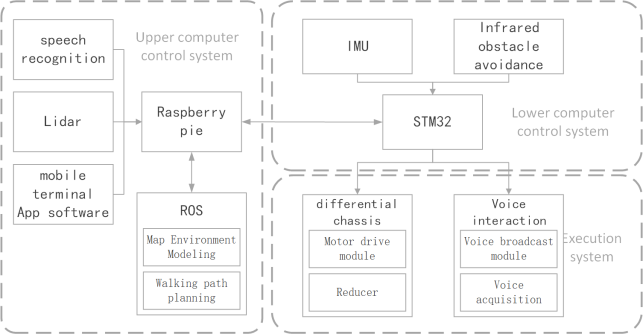
\includegraphics[width=4.8in ]{pics/stm32_pi.png}
    \caption{Composition block diagram of the entire system~\cite{kok2020intelligent}}
    \label{stm32_pi}
\end{figure}


\subsection{Summary of the literature review}

\end{comment}